\documentclass[11pt,a4paper]{article}

% ---------------------------------------------------------------------------
% Overlapping siphons, resident-dependent invasion, and uniform permanence
% in a two-strain coinfection reaction network.
%
% Author metadata: set the three macros below before submission.
% They are deliberately left blank in this version.
% ---------------------------------------------------------------------------
\newcommand{\PaperAuthor}{}
\newcommand{\PaperAffiliation}{}
\newcommand{\PaperDate}{14 September 2026}

\usepackage[T1]{fontenc}
\usepackage[utf8]{inputenc}
\usepackage{lmodern}
\usepackage{microtype}
\usepackage[a4paper,margin=1.05in]{geometry}
\usepackage{amsmath,amssymb,amsthm,mathtools}
\usepackage{booktabs}
\usepackage{array}
\usepackage{enumitem}
\usepackage{xcolor}
\usepackage{graphicx}
\usepackage[obeyspaces,spaces]{url}
\usepackage[numbers,sort&compress]{natbib}
\usepackage[colorlinks=true,linkcolor=blue!55!black,citecolor=blue!55!black,urlcolor=blue!55!black]{hyperref}
\hypersetup{pdftitle={Overlapping siphons, resident-dependent invasion, and uniform permanence in a two-strain coinfection reaction network},
  pdfkeywords={siphons, chemical reaction networks, uniform persistence, permanence, coinfection, multi-strain epidemic models, invasion, Lean}}

\DeclareUrlCommand\lean{\urlstyle{tt}}
\setlist{itemsep=2pt,topsep=3pt}
\setlength{\emergencystretch}{1.5em}
\graphicspath{{figures/}}

\theoremstyle{plain}
\newtheorem{theorem}{Theorem}[section]
\newtheorem{proposition}[theorem]{Proposition}
\newtheorem{lemma}[theorem]{Lemma}
\newtheorem{corollary}[theorem]{Corollary}
\theoremstyle{definition}
\newtheorem{definition}[theorem]{Definition}
\newtheorem{example}[theorem]{Example}
\theoremstyle{remark}
\newtheorem{remark}[theorem]{Remark}

\newcommand{\R}{\mathbb R}
\newcommand{\N}{\mathbb N}
\newcommand{\ch}{\chi}
\newcommand{\spb}{\mathfrak s}
\newcommand{\dd}{\mathrm d}
\newcommand{\eps}{\varepsilon}
\newcommand{\mat}[4]{\begin{pmatrix}#1&#2\\#3&#4\end{pmatrix}}
\newcommand{\cX}{\mathcal X}
\newcommand{\cA}{\mathcal A}
\newcommand{\cB}{\mathcal B}
\newcommand{\cE}{\mathcal E}
\DeclareMathOperator{\diag}{diag}
\DeclareMathOperator{\rank}{rank}
\DeclareMathOperator{\tr}{tr}

\title{Overlapping siphons, resident-dependent invasion,\\
and uniform permanence in a two-strain\\ coinfection reaction network}
\author{\PaperAuthor\\[2pt] {\small\itshape \PaperAffiliation}}
\date{\PaperDate}

\begin{document}
\maketitle

\begin{abstract}
A siphon of a reaction network is a set of species whose simultaneous absence is preserved by the dynamics. When two siphons overlap, the invasion of a shared species cannot be counted as two independent modes, and the linearization at a disease-free state does not determine whether an absent strain can invade a population in which the other strain is already resident. We address both issues for finite mass-action networks and for a specific four-compartment, fourteen-reaction two-strain coinfection model with constant recruitment.
The first result is structural: at any common boundary point of a family of siphons, first-order production can only decrease siphon membership, so the normal Jacobian is block triangular over membership signatures. For two siphons this yields the cross-multiplied characteristic identity $\ch_N\ch_{N_{S_1\cap S_2}}=\ch_{N_{S_1}}\ch_{N_{S_2}}$ on the fully covered normal space, valid as a polynomial identity and hence also at invasion thresholds.
The second result is dynamical: for the coinfection model, if all fourteen rates are positive, both single-strain resident equilibria exist, and each missing two-dimensional block strictly invades the other resident, then every positive initial state has a unique global positive solution, and there is a lower bound $\eps>0$, depending on the parameters but not on the initial state, that every compartment eventually exceeds. The converse holds away from the threshold: if one missing block is Hurwitz, that resident equilibrium attracts nearby positive states and permanence fails.
The proof derives the resident limits from an exactly corrected relative entropy, lifts the flow to a compact space of normalized infection masses, obtains one common growth window on the extinction boundary by compactness, and recovers each compartment from a product floor. An explicit example shows that the entire disease-free Jacobian can remain unchanged while resident invasion changes sign. The structural theorem and the permanence theorem, including existence and uniqueness, have warning-free Lean~4 proofs in a frozen Mathlib environment.
\end{abstract}

\section{Introduction}\label{sec:intro}

\subsection{Siphons, strains, and the overlap problem}

A siphon of a chemical reaction network is a set $S$ of species such that every reaction producing a species of $S$ consumes a species of $S$ \citep{AngeliDeLeenheerSontag2007,ShiuSturmfels2010,Feinberg2019}. If all species of a siphon are absent, they remain absent. Siphons are therefore the coordinate faces on which trajectories can accumulate, and the persistence theory of mass-action systems is organised around them: a bounded trajectory of a mass-action system fails to persist only by approaching a siphon face \citep{AngeliDeLeenheerSontag2007}, and much of the subsequent work on persistence and permanence of mass-action and power-law systems is an analysis of which siphons can actually be approached \citep{CraciunNazarovPantea2013}.

Avram, Adenane, Basnarkov and Horvath \citep{AvramAdenaneBasnarkovHorvath2025} observed that in compartmental epidemic models with several strains, the set of compartments carrying a given strain is a minimal siphon, and that the invasion of that strain into a disease-free population is governed by the normal linearization on that siphon face. When the strains do not share compartments, the siphons are disjoint, and the classical next-generation analysis \citep{DiekmannHeesterbeekMetz1990,vandenDriesscheWatmough2002} decouples strain by strain. In models with coinfection, a coinfected compartment carries both strains, the minimal siphons overlap, and the article \citep{AvramAdenaneBasnarkovHorvath2025} explicitly leaves the interpretation of the extra normal modes at an intersecting example for future work. A subsequent paper by Adenane, Avram and Halanay \citep{AdenaneAvramHalanay2026} proposes a conditional framework, in which persistence follows from a boundary Morse decomposition together with invasion inequalities at each boundary component, in the spirit of the acyclicity theorems of Butler, Freedman, Waltman, Hofbauer, So, Hale and Thieme \citep{ButlerFreedmanWaltman1986,ButlerWaltman1986,HofbauerSo1989,HaleWaltman1989,Garay1989,Thieme1993,FreedmanRuanTang1994,SmithThieme2011}. Related recent work by the same group treats non-interacting strains through Perron--Volterra Lyapunov functions \citep{AdenaneAvramBeldimanHalanay2026}, threshold theorems for balanced bilinear models \citep{AvramEtAl2026PerronFrobenius}, and relay transitions in multi-strain rumour models \citep{AvramAdenaneHalanay2026relay}.

Two distinct questions arise when siphons overlap.
\begin{enumerate}[label=(\roman*)]
\item \emph{Same resident state.} At a boundary point lying on the faces of both siphons, how do the normal matrices of the two siphons combine into the normal matrix of their union? A shared species is not two independent invading populations.
\item \emph{Different resident states.} Can invasion data computed at the disease-free equilibrium be transported to a face on which one strain is already resident? Here the answer is negative in general: a reaction that is quadratic in missing species at the disease-free state becomes linear in the missing strain once the other strain is present, and the invasion block itself changes.
\end{enumerate}
The present paper gives an exact answer to (i) for arbitrary finite mass-action networks, an explicit obstruction for (ii), and a complete permanence theorem, with converse, for a specific coinfection network in which the two minimal siphons overlap at a compartment that is not directly fed.

\subsection{Main results}

The structural result (Theorem~\ref{thm:overlap}) is that at a common boundary point $y$ of siphons $S_1,S_2$, the normal Jacobian $N$ on the full index set $S_1\cup S_2$ satisfies
\begin{equation}\label{eq:intro-overlap}
 \ch_N\,\ch_{N_I}=\ch_{N_{S_1}}\,\ch_{N_{S_2}},\qquad I=S_1\cap S_2,
\end{equation}
where $\ch_A(z)=\det(zI-A)$ and $N_S$ is the principal submatrix indexed by $S$. The shared factor is counted once. Since \eqref{eq:intro-overlap} is an identity of polynomials, nothing is divided by a determinant that may vanish at an invasion threshold. The underlying mechanism (Lemma~\ref{lem:membership}) is that a nonzero first-order production entry $N_{ij}$ forces the siphon membership of $i$ to be contained in that of $j$; for an arbitrary finite family of siphons this makes $N$ block triangular over membership signatures (Theorem~\ref{thm:signature}).

The dynamical result concerns the reduced coinfection model of \citep[Section~6]{AvramAdenaneBasnarkovHorvath2025} with constant recruitment, a four-compartment mass-action network with fourteen reactions and fourteen positive parameters (Table~\ref{tab:reactions}). Its minimal siphons are $\{a,c\}$ and $\{b,c\}$, where $a,b$ are the single-strain compartments and $c$ the coinfected compartment. Theorem~\ref{thm:main} states that if both single-strain resident equilibria $E_1,E_2$ exist and each missing two-dimensional block $M_1,M_2$ has a positive dominant eigenvalue, then every positive initial state has a unique global positive solution and there is $\eps>0$, depending only on the parameters, such that every such solution eventually satisfies $\eps\le s,a,b,c\le\Lambda/\mu_*+1$. Proposition~\ref{prop:converse} adds the converse away from the threshold: if $M_1$ or $M_2$ is Hurwitz, the corresponding resident equilibrium is locally asymptotically stable in the full system and permanence fails. Consequently, under positive rates, resident existence, and nonzero invasion eigenvalues, permanence holds if and only if both residents are strictly invadable (Corollary~\ref{cor:characterization}).

Two explicit computations delineate what information the criterion needs. In a one-parameter family (Example~\ref{ex:obstruction}), the disease-free reproduction numbers, the resident equilibria, and even the complete disease-free Jacobian are unchanged while the sign of the resident invasion eigenvalue changes. The invasion criterion is therefore not a function of any disease-free summary. A second computation (Section~\ref{sec:robust}) certifies strict mutual invasion, and hence permanence, on an entire box of parameters in which all fourteen rates vary independently by one percent around a reference point.

\subsection{Method}

The permanence proof does not invoke a general acyclic-boundary theorem. It proves the required uniform repulsion directly for this source, in a form that controls repeated returns to the extinction boundary and not merely local escape from each equilibrium. The steps are as follows.
\begin{enumerate}
\item A total-population balance gives global existence, strict positivity, and an absorbing box; an exactly corrected relative entropy proves convergence of every single-strain trajectory to its resident equilibrium, without assuming a positive infected floor and with unequal mortality rates (Section~\ref{sec:boundary}).
\item Strict invasion of each resident yields positive covectors and weighted missing masses $U=a+r_uc$ and $V=b+r_vc$; a third mass $J=a+b+r_jc$ and an integer power $k$ compensate the disease-free equilibrium, where the two resident weights alone give no sign information. The quantity of interest is the product $P=UVJ^k$ (Section~\ref{sec:lift}).
\item The relative growth rate of $P$ is singular on the extinction faces. Adjoining the normalized coordinates $a/U,b/V,a/J,b/J$ produces a polynomial vector field on $\R^8$ whose physical trajectories lie in a compact set $K$, the closure of the normalized positive states. The relative growth $G$ of $P$ is continuous on $K$ and $\dot P=GP$ there, including at $P=0$.
\item On the extinction set $Z=\{P=0\}\subset K$, every projection converges to $E_0$, $E_1$, or $E_2$, and $G$ is strictly positive on the compact fiber over each of these equilibria. Compactness converts this into one common integer time $N$ with accumulated growth $\cA(z,N)>1$ for all $z\in Z$ (Section~\ref{sec:window}).
\item Continuity extends the window to a collar $\{P\le\rho\}$, a sampled comparison gives an eventual floor for $P$ that is independent of the trajectory, and bounded relative loss controls the dips between samples. Individual compartments are then recovered by exact forcing identities (Section~\ref{sec:recovery}).
\end{enumerate}
The role of compactness is to supply the existence of the floor; no simulated minimum enters the argument, and the constants of the recovery step are explicit formulas in the compactness-derived product floor.

\subsection{Scope and formal verification}

The theorems are stated for the literal network of Table~\ref{tab:reactions}. We do not claim a permanence theorem for arbitrary networks with overlapping siphons, and the structural identity \eqref{eq:intro-overlap} is a statement about one boundary point: it does not multiply the spectra of $M_1$ at $E_1$ and $M_2$ at $E_2$. The hypotheses of Theorem~\ref{thm:main} exclude zero rates and zero invasion eigenvalues; the threshold case, global convergence of interior solutions, an effective general value of $\eps$, and a floor that is uniform over a parameter box are not claimed (Section~\ref{sec:discussion}).

The structural theorem, the permanence theorem with existence and uniqueness, the two-dimensional invasion criteria, and the one-percent parameter-box certificate have been formalized in Lean~4 \citep{deMouraUllrich2021} over a frozen Mathlib \citep{mathlib2020} snapshot, compiled with every warning treated as an error, and checked to depend only on the standard axioms. Section~\ref{sec:formal} maps the mathematical steps to the formal declarations and states precisely which statements of this paper are conventional (Proposition~\ref{prop:converse}, Remarks~\ref{rem:splitting} and \ref{rem:signature-refinement}). The mathematical proofs below are complete and independent of the formal development.

\subsection{Organization}

Section~\ref{sec:model} fixes the network and states the main theorems. Section~\ref{sec:structure} proves the membership lemma and the overlap identities. Section~\ref{sec:invasion} treats two-dimensional invasion, the obstruction example, and the converse. Sections~\ref{sec:boundary}--\ref{sec:recovery} prove Theorem~\ref{thm:main}. Section~\ref{sec:robust} records the parameter-box certificate, Section~\ref{sec:discussion} discusses scope and open questions, and Section~\ref{sec:formal} describes the formal verification.

\section{The reaction network and the main theorems}\label{sec:model}

Write $x=(s,a,b,c)\in\R_{\ge0}^4$ for the densities of susceptible individuals, individuals infected only with strain~1, individuals infected only with strain~2, and coinfected individuals. Table~\ref{tab:reactions} lists the fourteen reactions; each contributes its product-minus-reactant vector multiplied by the indicated mass-action rate. This is the constant-recruitment version of the reduced coinfection model in \citep[Section~6]{AvramAdenaneBasnarkovHorvath2025}; compartmental coinfection models of this type go back at least to \citep{MartchevaPilyugin2006,GaoPorcoRuan2016}.

\begin{table}[ht]
\centering
\caption{The fourteen reactions and their mass-action rates.}\label{tab:reactions}
\begin{tabular}{cll@{\qquad}cll}
\toprule
 & Reaction & Rate & & Reaction & Rate\\
\midrule
1 & $\varnothing\to s$ & $\Lambda$ & 8 & $a+b\to a+c$ & $\gamma_2ab$\\
2 & $s+a\to2a$ & $\alpha_1sa$ & 9 & $s+c\to a+c$ & $\beta_1sc$\\
3 & $s+b\to2b$ & $\alpha_2sb$ & 10 & $s+c\to b+c$ & $\beta_2sc$\\
4 & $s+c\to2c$ & $\alpha_3sc$ & 11 & $s\to\varnothing$ & $\mu_0s$\\
5 & $a+c\to2c$ & $\eta_1ac$ & 12 & $a\to\varnothing$ & $\mu_1a$\\
6 & $b+c\to2c$ & $\eta_2bc$ & 13 & $b\to\varnothing$ & $\mu_2b$\\
7 & $a+b\to b+c$ & $\gamma_1ab$ & 14 & $c\to\varnothing$ & $\mu_3c$\\
\bottomrule
\end{tabular}
\end{table}

If density has unit $D$ and time has unit $T$, then $\Lambda$ has unit $D/T$, each $\mu_i$ has unit $T^{-1}$, and all $\alpha_i,\beta_i,\gamma_i,\eta_i$ have unit $D^{-1}T^{-1}$. All fourteen parameters are strictly positive. The loss rates may aggregate mortality and permanent removal; recovery and immunity are not tracked and there is no return to susceptibility. Reactions~9 and~10 describe the transmission of a single strain by a coinfected individual, reactions~5 and~6 the superinfection of a single-strain carrier by a coinfected one, and reactions~7 and~8 the superinfection of one single-strain carrier by the other. The theorems are properties of this source, without a calibration or treatment interpretation.

The differential equations are
\begin{equation}\label{eq:ode}
\begin{aligned}
 \dot s&=\Lambda-s\bigl[\mu_0+\alpha_1a+\alpha_2b+(\alpha_3+\beta_1+\beta_2)c\bigr],\\
 \dot a&=a(\alpha_1s-\gamma_1b-\eta_1c-\mu_1)+\beta_1sc,\\
 \dot b&=b(\alpha_2s-\gamma_2a-\eta_2c-\mu_2)+\beta_2sc,\\
 \dot c&=(\gamma_1+\gamma_2)ab+c(\eta_1a+\eta_2b+\alpha_3s-\mu_3).
\end{aligned}
\end{equation}
Let
\begin{equation}\label{eq:residents}
 s_0=\frac{\Lambda}{\mu_0},\qquad s_i=\frac{\mu_i}{\alpha_i},\qquad
 u_i=\frac{\Lambda-\mu_0s_i}{\mu_i}\quad(i=1,2).
\end{equation}
Assume $s_i<s_0$ for $i=1,2$. Then $u_i>0$, and the three boundary equilibria are
\[
 E_0=(s_0,0,0,0),\qquad E_1=(s_1,u_1,0,0),\qquad E_2=(s_2,0,u_2,0).
\]
The condition $s_i<s_0$ is $\alpha_is_0/\mu_i>1$, the classical threshold for strain $i$ alone. At $E_1$ the missing variables are $(b,c)$; at $E_2$ they are $(a,c)$. Differentiating \eqref{eq:ode} gives their normal matrices
\begin{equation}\label{eq:blocks}
\begin{split}
 M_1&=\mat{\alpha_2s_1-\gamma_2u_1-\mu_2}{\beta_2s_1}
                  {(\gamma_1+\gamma_2)u_1}{\eta_1u_1+\alpha_3s_1-\mu_3},\\[3pt]
 M_2&=\mat{\alpha_1s_2-\gamma_1u_2-\mu_1}{\beta_1s_2}
                  {(\gamma_1+\gamma_2)u_2}{\eta_2u_2+\alpha_3s_2-\mu_3}.
\end{split}
\end{equation}
Both off-diagonal entries of each matrix are strictly positive: the coinfected compartment produces the missing single-strain compartment through the $\beta$ reactions, and the resident strain produces coinfected individuals from the missing strain through the $\gamma$ reactions. The latter reaction is quadratic in the missing species at $E_0$ and linear at $E_1$ and $E_2$; this is the resident-dependent activation discussed in the introduction. For a real square matrix $M$, $\spb(M)$ denotes the maximum real part of its eigenvalues.

\begin{theorem}[Uniform species permanence]\label{thm:main}
Suppose all fourteen parameters in \eqref{eq:ode} are positive, $s_1<s_0$, $s_2<s_0$, and $\spb(M_1)>0$, $\spb(M_2)>0$. Then every $x_0\in\R_{>0}^4$ admits a global positive forward solution, unique on $t\ge0$. There is $\eps>0$, depending only on the parameters, such that every such solution satisfies, for all sufficiently large $t$,
\begin{equation}\label{eq:permanence}
 \eps\le s(t),a(t),b(t),c(t)\le\frac{\Lambda}{\mu_*}+1,
 \qquad \mu_*:=\min_{0\le i\le3}\mu_i.
\end{equation}
The time after which \eqref{eq:permanence} holds may depend on $x_0$; $\eps$ does not.
\end{theorem}

The constant $1$ in the upper bound is one chosen density unit; any fixed positive margin above $\Lambda/\mu_*$ can be used instead. The theorem asserts permanence, not convergence of the interior flow to an equilibrium, and it imposes no relation between the four mortality rates.

\begin{theorem}[Full-cover overlap identity]\label{thm:overlap}
Let $S_1,S_2$ be siphons of a finite mass-action network with positive rate constants, let $y$ be a point of the nonnegative orthant with $y_i=0$ for all $i\in S_1\cup S_2$, and let $N$ be the Jacobian of the mass-action field at $y$ restricted to the rows and columns indexed by $S_1\cup S_2$. Write $N_S$ for the principal submatrix indexed by $S$ and $I=S_1\cap S_2$. Then, as polynomials,
\[
 \ch_N\,\ch_{N_I}=\ch_{N_{S_1}}\,\ch_{N_{S_2}},
\]
where the characteristic polynomial of an empty matrix is $1$.
\end{theorem}

Theorem~\ref{thm:overlap} is proved in Section~\ref{sec:structure} together with its finite-family generalization; Theorem~\ref{thm:main} is proved in Sections~\ref{sec:boundary}--\ref{sec:recovery}. The converse direction, Proposition~\ref{prop:converse}, is proved in Section~\ref{sec:invasion}.

\section{Siphon membership and overlap composition}\label{sec:structure}

Consider a finite mass-action network with species set $\cX$, reactions $y_r\to y'_r$ with reactant and product vectors $y_r,y'_r\in\N^{\cX}$, positive rate constants $k_r$, and polynomial vector field
\begin{equation}\label{eq:massaction}
 f_i(x)=\sum_r k_r\,(y'_{ri}-y_{ri})\prod_{j\in\cX}x_j^{y_{rj}},\qquad i\in\cX.
\end{equation}
A set $S\subseteq\cX$ is a \emph{siphon} if every reaction with $y'_{ri}>y_{ri}$ for some $i\in S$ has $y_{rj}>0$ for some $j\in S$. Its coordinate face is $F_S=\{x\in\R^{\cX}_{\ge0}:x_i=0\text{ for all }i\in S\}$. Note that $F_{S_1}\cap F_{S_2}=F_{S_1\cup S_2}$, and that a union of siphons is a siphon, whereas an intersection of siphons need not be one.

\begin{lemma}[Source-derived membership zeros]\label{lem:membership}
Let $S_1,\ldots,S_m$ be siphons, let $y\in\bigcap_\ell F_{S_\ell}$, and set $N_{ij}=\partial_jf_i(y)$. Define the membership signature $m(i)=\{\ell:i\in S_\ell\}$. Then
\begin{equation}\label{eq:membership}
 N_{ij}\ne0\quad\Longrightarrow\quad m(i)\subseteq m(j).
\end{equation}
Moreover $N_{ij}\ge0$ whenever $i\ne j$ both lie in $\bigcup_\ell S_\ell$.
\end{lemma}
\begin{proof}
Let $S$ be a siphon containing $i$. Every reaction contributing a nonzero term to $f_i$ consumes a species of $S$: if the reaction produces $i$ this is the siphon property, and if it consumes $i$ then $i$ itself is a reactant. Hence every monomial of $f_i$ contains a factor $x_j$ with $j\in S$, and $f_i$ vanishes identically on $F_S$. If $j\notin S$, the line $t\mapsto y+te_j$ stays in $F_S$, so $\partial_jf_i(y)=0$. Applying this to every siphon containing $i$ proves \eqref{eq:membership}. For the sign statement, let $i\ne j$ be missing at $y$. Every reaction producing $i$ with nonzero rate along $y+te_j$, $t>0$, has $y_{ri}=0$ (all other missing coordinates are zero), so its stoichiometric coefficient $y'_{ri}-y_{ri}\ge0$; reactions consuming $i$ contribute zero because $y_i=0$ along the line. Thus $f_i(y+te_j)\ge0$ for $t\ge0$, and since $f_i(y)=0$ the derivative is nonnegative.
\end{proof}

The proof uses a polynomial identity on the entire coordinate face, not a derivative sign read off a reaction graph. The sign statement is the familiar Metzler property of normal Jacobians; the containment \eqref{eq:membership} is the structural input.

\begin{theorem}[Signature factorization]\label{thm:signature}
In the setting of Lemma~\ref{lem:membership}, let $N$ be the Jacobian restricted to a set $Z\supseteq\bigcup_\ell S_\ell$ of coordinates vanishing at $y$, and for each integer $q$ let $B_q=\{i\in Z:|m(i)|=q\}$. Then $N$ is block upper triangular with respect to the ordering of $Z$ by decreasing $|m(i)|$, and
\begin{equation}\label{eq:card-factor}
 \ch_N=\prod_{q}\ch_{N_{B_q}}.
\end{equation}
\end{theorem}
\begin{proof}
If $N_{ij}\ne0$ then $m(i)\subseteq m(j)$ by \eqref{eq:membership}, hence $|m(i)|\le|m(j)|$. Thus every nonzero entry of $N$ lies on or above the block diagonal when rows and columns are grouped by decreasing cardinality, and the characteristic polynomial of a block triangular matrix is the product of those of its diagonal blocks.
\end{proof}

\begin{remark}[Refinement by signature]\label{rem:signature-refinement}
Within a cardinality class $B_q$, two coordinates with distinct signatures have incomparable signatures, so by \eqref{eq:membership} the entries between them vanish in both directions. Hence each diagonal block $N_{B_q}$ is block diagonal over signatures and \eqref{eq:card-factor} refines to $\ch_N=\prod_T\ch_{N_{B_T}}$ over the realized signatures $T$, with $B_T=\{i:m(i)=T\}$. If the siphons do not cover $Z$, the empty signature $T=\varnothing$ contributes a factor that must be retained: an uncovered coordinate may carry a normal mode. If the siphons are pairwise disjoint and cover $Z$, then $N$ is block diagonal over the siphons and $\spb(N)=\max_\ell\spb(N_{S_\ell})$. For a general covering family, every signature block lies inside at least one $S_\ell$, and $N_{S_\ell}$ has the corresponding triangular subcollection of blocks, so again $\spb(N)=\max_\ell\spb(N_{S_\ell})$. These refinements are immediate from Theorem~\ref{thm:signature}; only the cardinality version \eqref{eq:card-factor} and the two-siphon identity below are among the compiled declarations of Section~\ref{sec:formal}.
\end{remark}

\begin{proof}[Proof of Theorem~\ref{thm:overlap}]
Write $U=S_1\setminus S_2$ and $V=S_2\setminus S_1$. Then $U,V,I$ partition $S_1\cup S_2$, with signatures $\{1\}$, $\{2\}$, $\{1,2\}$. Ordering the coordinates as $(U,V,I)$, Lemma~\ref{lem:membership} gives
\begin{equation}\label{eq:triangular}
 N=\begin{pmatrix}N_U&0&*\\0&N_V&*\\0&0&N_I\end{pmatrix}.
\end{equation}
Consequently $\ch_N=\ch_{N_U}\ch_{N_V}\ch_{N_I}$, $\ch_{N_{S_1}}=\ch_{N_U}\ch_{N_I}$, and $\ch_{N_{S_2}}=\ch_{N_V}\ch_{N_I}$. Multiplying the last two identities and comparing with the first proves the claim.
\end{proof}

The cover condition is essential to the normal-space interpretation: a coordinate missing at $y$ but in neither siphon belongs to a further block and cannot be omitted from a claim about a larger normal space. All matrices in Theorem~\ref{thm:overlap} are evaluated at the same point $y$. In particular the formula does not combine $M_1(E_1)$ with $M_2(E_2)$, which live at different residents; the relation between those two matrices and permanence is the subject of Sections~\ref{sec:invasion}--\ref{sec:recovery}.

\begin{remark}[Regular splittings]\label{rem:splitting}
Next-generation analysis \citep{DiekmannHeesterbeekMetz1990,vandenDriesscheWatmough2002} writes a normal matrix as $N=F-V$ with $F\ge0$ entrywise and $V$ a nonsingular M-matrix, and identifies the sign of $\spb(N)$ with the sign of $\rho(FV^{-1})-1$ \citep{BermanPlemmons1994}. A structural zero $N_{ij}=0$ with $i\ne j$ forces $F_{ij}=0$ and $V_{ij}=0$, since $F_{ij}\ge0$ and $-V_{ij}\ge0$. Hence $F$ and $V$ inherit the block triangular pattern of Theorem~\ref{thm:signature}, and so do $V^{-1}$ and $K=FV^{-1}$: the diagonal blocks of $V^{-1}$ are the inverses of the diagonal blocks of $V$, each again a nonsingular M-matrix with nonnegative inverse, and the block inverse recursion only follows chains of permitted inclusions. Therefore $K_T=F_T V_T^{-1}$ blockwise and $\rho(K)=\max_T\rho(K_T)$. This transfers the factorization to next-generation matrices for any regular splitting; the numerical values of the resulting reproduction numbers depend on the splitting, whereas the threshold does not. The scalar implication $N_{ij}=0\Rightarrow F_{ij}=V_{ij}=0$ is among the compiled declarations; the remaining statements of this remark are standard matrix theory and are not formalized here.
\end{remark}

\paragraph{The concrete instance.}
For Table~\ref{tab:reactions}, a nonempty siphon cannot contain $s$, because reaction~1 produces $s$ from nothing. If it contains $a$ or $b$, reaction~9 or~10 (which produces $a$ or $b$ from $s$ and $c$) forces it to contain $c$. If it contains $c$, reaction~7 (which produces $c$ from $a$ and $b$) forces it to contain $a$ or $b$. Checking the reactionwise condition for the remaining candidates shows that the siphons are exactly
\begin{equation}\label{eq:siphons}
 \varnothing,\qquad S_1=\{a,c\},\qquad S_2=\{b,c\},\qquad S_1\cup S_2=\{a,b,c\}.
\end{equation}
The two minimal siphons overlap at $c$, which is not directly fed, and their intersection $\{c\}$ is not a siphon. At $y=(s,0,0,0)$, any $s\ge0$, the normal matrix on $(a,b,c)$ is
\begin{equation}\label{eq:dfe-normal}
 N(s)=\begin{pmatrix}
 \alpha_1s-\mu_1&0&\beta_1s\\
 0&\alpha_2s-\mu_2&\beta_2s\\
 0&0&\alpha_3s-\mu_3
 \end{pmatrix},
\end{equation}
so $\ch_N=(z-\alpha_1s+\mu_1)(z-\alpha_2s+\mu_2)(z-\alpha_3s+\mu_3)$, $\ch_{N_{S_1}}=(z-\alpha_1s+\mu_1)(z-\alpha_3s+\mu_3)$, and $\ch_{N_{S_2}}=(z-\alpha_2s+\mu_2)(z-\alpha_3s+\mu_3)$. The shared factor $z-(\alpha_3s-\mu_3)$ occurs once in $\ch_N$ and once in each siphon polynomial, as Theorem~\ref{thm:overlap} requires. At $E_0$ there are three normal modes although there are only two minimal siphons; the shared mode can feed both private modes through the $\beta$ entries, but no private mode can feed the shared mode: the reaction $a+b\to b+c$ that produces $c$ from private species is quadratic and disappears from the linearization at $E_0$. It reappears, linearly, at $E_1$ and $E_2$, which is why \eqref{eq:blocks} has positive lower-left entries.

\begin{figure}[ht]
\centering
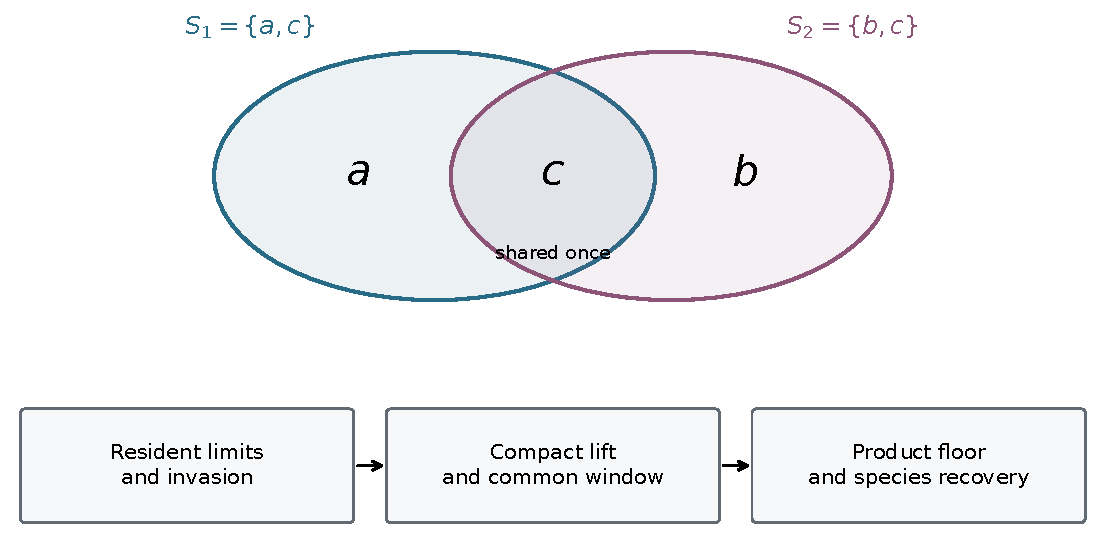
\includegraphics[width=.88\textwidth]{proof_structure.pdf}
\caption{The two minimal siphons of the coinfection network share the coinfected compartment $c$, which is counted once in the normal characteristic polynomial. The lower row summarizes the permanence proof: resident limits and strict invasion are transferred through a compact normalized flow to a product floor, from which the individual compartments are recovered.}
\label{fig:structure}
\end{figure}

\section{Resident-dependent invasion}\label{sec:invasion}

\subsection{Two-dimensional criteria without a spectral black box}

\begin{lemma}[Two-dimensional strict invasion and strict stability]\label{lem:covector}
Let $M=\mat ABCD$ with $B,C>0$, and let $\lambda_+(M)=\bigl(A+D+\sqrt{(A-D)^2+4BC}\bigr)/2$ be its larger eigenvalue, which is real and exceeds both diagonal entries.
\begin{enumerate}[label=(\alph*)]
\item The following are equivalent: $\lambda_+(M)>0$; \ $A\ge0$ or $D\ge0$ or $AD<BC$; \ there is $r>0$ with $A+rC>0$ and $B+rD>0$. When they hold, $\delta=\tfrac12\min\{A+rC,(B+rD)/r\}>0$ satisfies $(1,r)M\ge2\delta\,(1,r)$ componentwise.
\item The following are equivalent: $\lambda_+(M)<0$; \ $A<0$, $D<0$ and $BC<AD$; \ there is $r>0$ with $A+rC<0$ and $B+rD<0$.
\end{enumerate}
\end{lemma}
\begin{proof}
Since $\sqrt{(A-D)^2+4BC}>|A-D|$, $\lambda_+$ exceeds $\max(A,D)$. If $A,D<0$, then $\lambda_+>0$ if and only if $(A-D)^2+4BC>(A+D)^2$, that is $BC>AD$; and $\lambda_+<0$ if and only if $BC<AD$. This proves the first equivalence in each part. For (a), if $D\ge0$ then $B+rD>0$ for every $r>0$ and $A+rC>0$ for all large $r$. If $D<0$, the second condition implies $AD<BC$ (trivially if $A\ge0$), and $A+rC>0$, $B+rD>0$ hold exactly for $\max\{0,-A/C\}<r<B/(-D)$, an interval that is nonempty precisely when $AD<BC$. Conversely, if $r$ exists and $D<0$, multiplying $A+rC>0$ by $-D>0$ and $B+rD>0$ by $C>0$ and adding gives $-AD+BC>0$. The margin $\delta$ is immediate. For (b), if $A+rC<0$ and $B+rD<0$ with $r>0$ then $A<0$ and $D<0$, and multiplying by $-D$ and $C$ as before gives $BC<AD$; conversely $A,D<0$ and $BC<AD$ make the interval $B/(-D)<r<(-A)/C$ nonempty.
\end{proof}

The lemma replaces a spectral computation by two rational inequalities, and for rational parameters it produces a rational certificate $(1,r)$. Both parts are compiled declarations (Section~\ref{sec:formal}). The permanence hypothesis of Theorem~\ref{thm:main} is used in the form (a) for $M_1$ and $M_2$; when both diagonal entries are negative, it says that the loop gain $BC/(AD)$ of the two-step cycle ``missing single-strain compartment $\to$ coinfected compartment $\to$ missing single-strain compartment'' exceeds one.

\subsection{The disease-free state does not determine resident invasion}

\begin{example}[Same disease-free data, opposite invasion outcomes]\label{ex:obstruction}
Take
\begin{gather*}
 \Lambda=4,\qquad \mu_0=\mu_1=\mu_2=\mu_3=1,\qquad
 (\alpha_1,\alpha_2,\alpha_3)=(2,1,1),\
 \eta_1=\eta_2=\gamma_1=\gamma_2=\beta_1=\tfrac1{10},
\end{gather*}
and leave $\beta_2>0$ free. All fourteen rates are positive, $s_0=4$, $E_1=(\tfrac12,\tfrac72,0,0)$, $E_2=(1,0,3,0)$, and the disease-free reproduction numbers $\alpha_is_0/\mu_i$ are $(8,4,4)$, independent of $\beta_2$. The resident matrices are
\[
 M_1=\mat{-17/20}{\beta_2/2}{7/10}{-3/20},\qquad
 M_2=\mat{7/10}{1/10}{3/5}{3/10},
\]
so $\det M_1=\tfrac{51}{400}-\tfrac{7}{20}\beta_2$ and, by Lemma~\ref{lem:covector}, $M_1$ strictly invades exactly when $\beta_2>\beta_2^*:=51/140$, while $M_2$ strictly invades for every $\beta_2$ (its upper-left entry is positive; the covector $(1,1)$ gives $(1,1)M_2=(\tfrac{13}{10},\tfrac25)$). At $\beta_2=\tfrac1{10}$ the eigenvalue $\lambda_+(M_1)=\bigl(-1+\sqrt{\tfrac{49}{100}+\tfrac{7}{5}\beta_2}\bigr)/2\approx-0.103$ is negative and the stable covector $(1,5)$ gives $M_1(1,5)^{\mathsf T}=(-\tfrac35,-\tfrac1{20})^{\mathsf T}$; at $\beta_2=1$ it is $\approx0.187$ and $(1,2)M_1=(\tfrac{11}{20},\tfrac15)\ge\tfrac1{10}(1,2)$. Thus both parameter choices have the same siphons, the same resident equilibria and the same disease-free reproduction numbers, but at $\beta_2=\tfrac1{10}$ strain~2 cannot invade the strain-1 resident, whereas at $\beta_2=1$ Theorem~\ref{thm:main} applies and both strains persist uniformly.

A stronger obstruction uses the superinfection rate. Fix $\beta_2=\tfrac1{10}$ and change $\eta_1$ from $\tfrac1{10}$ to $\tfrac15$. The terms containing $\eta_1$ are quadratic in $(a,c)$, so the entire $4\times4$ Jacobian at $E_0$ is unchanged, and so is $E_1$. The new resident matrix is
\[
 \mat{-17/20}{1/20}{7/10}{1/5},\qquad \det=-\tfrac{41}{200}<0,
\]
which strictly invades. Hence even the complete disease-free linearization does not determine whether the resident state $E_1$ can be invaded; the missing information is the resident-dependent activation of the reactions $a+c\to2c$ and $a+b\to b+c$.
\end{example}

The threshold determinant $\det M_1=\tfrac{51}{400}-\tfrac{7}{20}\beta_2$ of this family is a compiled declaration; the remaining arithmetic of the example is elementary and is recorded here in exact form so that it can be rechecked by hand.

\subsection{The converse: a Hurwitz block excludes permanence}

\begin{proposition}[Local attraction of an uninvadable resident]\label{prop:converse}
Assume all rates positive and $s_1<s_0$. If $\spb(M_1)<0$, then $E_1$ is a hyperbolic sink of \eqref{eq:ode}: there is a neighbourhood of $E_1$ in $\R^4$ from which every solution converges to $E_1$. This neighbourhood contains positive states, along whose solutions $b(t),c(t)\to0$. Consequently no $\eps>0$ can satisfy \eqref{eq:permanence} for all positive solutions, and permanence fails. The same holds for $E_2$ when $\spb(M_2)<0$.
\end{proposition}
\begin{proof}
In the order $(s,a,b,c)$, the Jacobian of \eqref{eq:ode} at $E_1$ is
\[
 J(E_1)=\begin{pmatrix}T&*\\0&M_1\end{pmatrix},\qquad
 T=\mat{-(\mu_0+\alpha_1u_1)}{-\mu_1}{\alpha_1u_1}{0},
\]
because $\partial_s\dot b=\alpha_2b+\beta_2c$, $\partial_a\dot b=-\gamma_2b$, $\partial_s\dot c=\alpha_3c$ and $\partial_a\dot c=(\gamma_1+\gamma_2)b+\eta_1c$ all vanish at $b=c=0$, and $\partial_a\dot a=\alpha_1s_1-\mu_1=0$ at the resident. The tangent block $T$ has trace $-(\mu_0+\alpha_1u_1)<0$ and determinant $\alpha_1\mu_1u_1>0$, so both of its eigenvalues have negative real part. With $\spb(M_1)<0$ all four eigenvalues of $J(E_1)$ have negative real part. By the linearization theorem for hyperbolic equilibria (Lyapunov's first method), $E_1$ is locally asymptotically stable in $\R^4$, and every solution starting in a suitable ball around $E_1$ converges to $E_1$. Since $s_1,u_1>0$, this ball contains points of $\R^4_{>0}$; the corresponding solutions remain positive for all forward time (Lemma~\ref{lem:absorber} below, which uses only positivity of the rates) and have $b(t)+c(t)\to0$, so \eqref{eq:permanence} fails for every $\eps>0$.
\end{proof}

\begin{corollary}[Strict characterization]\label{cor:characterization}
Assume all fourteen rates positive, $s_1<s_0$, $s_2<s_0$, and $\spb(M_1)\ne0\ne\spb(M_2)$. Then the conclusion of Theorem~\ref{thm:main} holds if and only if $\spb(M_1)>0$ and $\spb(M_2)>0$.
\end{corollary}

The corollary says nothing about the threshold strata $\spb(M_i)=0$, about parameters with $s_i\ge s_0$ (where a resident is absent and the boundary structure changes), or about zero rates (which change the reaction support and hence the siphons). Proposition~\ref{prop:converse} is a conventional argument and is not among the compiled declarations; its linear-algebraic ingredients, the identity $\tr T<0<\det T$ and the equivalence in Lemma~\ref{lem:covector}(b), are formalized.

\section{Boundary dynamics}\label{sec:boundary}

We now begin the proof of Theorem~\ref{thm:main}. Throughout Sections~\ref{sec:boundary}--\ref{sec:recovery}, all fourteen rates are positive. The resident existence and invasion hypotheses are used only from Section~\ref{sec:lift} onward. The boundary limits derived in this section are conclusions, not hypotheses.

\begin{lemma}[Global flow and absorption]\label{lem:absorber}
Every nonnegative initial state has a global nonnegative forward solution of \eqref{eq:ode}, unique on $t\ge0$. Initially positive coordinates remain positive. Every solution eventually enters and stays in
\[
 \cB_R=\{x\ge0:s+a+b+c\le R\},\qquad R=\Lambda/\mu_*+1.
\]
There is also a positive eventual lower bound $\ell$ for $s$, independent of the initial state.
\end{lemma}
\begin{proof}
The polynomial field is locally Lipschitz, and each $f_i$ is nonnegative on the part of the nonnegative orthant where $x_i=0$, so the orthant is forward invariant for the maximal solution. For $n=s+a+b+c$, all contact terms cancel and
\begin{equation}\label{eq:balance}
 \dot n=\Lambda-\mu_0s-\mu_1a-\mu_2b-\mu_3c\le\Lambda-\mu_*n.
\end{equation}
Scalar comparison gives $n(t)\le\max\{n(0),\Lambda/\mu_*\}$ for all $t$ in the maximal interval, so the solution stays bounded and is global, and gives eventual entry into $\cB_R$. On a bounded set every coordinate satisfies $\dot x_i\ge-Cx_i$ for some finite $C$, so an initially positive coordinate remains positive; this is the comparison $x_i(t)\ge x_i(0)e^{-Ct}$. Uniqueness on $[0,T]$ follows from the local Lipschitz property on the bounded set containing the trajectory, for every finite $T$. Finally, set
\begin{equation}\label{eq:s-floor}
 Q=\mu_0+(\alpha_1+\alpha_2+\alpha_3+\beta_1+\beta_2)R,\qquad \ell=\frac{\Lambda}{2Q}>0.
\end{equation}
Once the solution is in $\cB_R$, $\dot s\ge\Lambda-Qs$, and comparison gives $s(t)\ge\ell$ for all large $t$, even when $s(0)=0$.
\end{proof}

The identity \eqref{eq:balance} is a total-population balance; it is not a conservation law, since recruitment and removal are open channels.

\begin{lemma}[Resident convergence]\label{lem:resident}
Assume $s_1<s_0$. On the face $b=c=0$, every solution with $a(0)>0$ converges to $E_1$. Symmetrically, if $s_2<s_0$, on $a=c=0$ every solution with $b(0)>0$ converges to $E_2$. On $a=b=c=0$ every solution converges to $E_0$.
\end{lemma}
\begin{proof}
On either single-strain face write the positive variables as $(s,u)$ and the parameters as $(\alpha,\mu)$. The equations are
\[
 \dot s=\Lambda-\mu_0s-\alpha su,\qquad \dot u=\alpha su-\mu u.
\]
Let $(\bar s,\bar u)$ be the positive resident ($\alpha\bar s=\mu$, $\Lambda=\mu_0\bar s+\alpha\bar s\bar u$), and set $g=\mu_0+\alpha\bar u$, $v=s-\bar s$, $w=u-\bar u$. Substituting, $\dot s=-gv-\alpha sw$ and $\dot u=\alpha uv$. For positive $s,u$ define the relative entropy
\[
 H=s-\bar s-\bar s\log(s/\bar s)+u-\bar u-\bar u\log(u/\bar u)\ge0.
\]
Direct differentiation gives $\dot H=(v/s)\dot s+(w/u)\dot u=-gv^2/s$, in which the cross terms $\mp\alpha vw$ cancel. This is only semidefinite. Consider the corrected function $H_\eps=H+\eps vw$; since $\frac{\dd}{\dd t}(vw)=\dot sw+v\dot u$, its derivative is exactly
\begin{equation}\label{eq:strict-entropy}
 \dot H_\eps=-\Bigl(\frac gs-\eps\alpha u\Bigr)v^2-\eps gvw-\eps\alpha sw^2.
\end{equation}
By Lemma~\ref{lem:absorber}, eventually $\ell\le s\le R$ and $u\le R$. Choose $\eps>0$ so small that
\[
 \eps\alpha R\le\frac{g}{4R},\qquad \eps gR\le\frac{\alpha\ell}{2}.
\]
Then $g/s-\eps\alpha u\ge3g/(4R)$, and writing $-\eps gvw=-\frac{g}{4R}(v+2\eps Rw)^2+\frac{g}{4R}v^2+g\eps^2Rw^2$ in \eqref{eq:strict-entropy} gives
\begin{equation}\label{eq:strict-drift}
 \dot H_\eps\le-\frac{g}{2R}v^2-\frac{\eps\alpha\ell}{2}w^2 .
\end{equation}
Since $H\ge0$ and $|\eps vw|$ is bounded on the box, $H_\eps$ is bounded below, so \eqref{eq:strict-drift} gives $\int^\infty(v^2+w^2)\,\dd t<\infty$. The vector field is bounded on the box, so $v^2+w^2$ is uniformly continuous in $t$, and a nonnegative uniformly continuous integrable function tends to zero (otherwise infinitely many disjoint intervals of fixed length on which it exceeds a fixed positive value would force an infinite integral). Hence $(s,u)\to(\bar s,\bar u)$. If $s(0)=0$, positivity of $s$ for $t>0$ follows from recruitment and the argument applies after a time shift; positivity of $u$ was proved in Lemma~\ref{lem:absorber} and is not an eventual-floor assumption. On the disease-free line $\dot s=\Lambda-\mu_0s$, which converges to $s_0$.
\end{proof}

The correction term is what makes the proof work for unequal mortality rates. With $\mu_0=\mu_i$ the total population on the face converges to a constant and the resident system reduces to one dimension; without that identity, the classical entropy alone yields only the semidefinite drift $-gv^2/s$, and the corrected entropy \eqref{eq:strict-entropy} restores a strictly negative definite quadratic form on the absorbing box.

\section{A compact normalized flow}\label{sec:lift}

Assume now $s_1<s_0$, $s_2<s_0$, $\spb(M_1)>0$ and $\spb(M_2)>0$. Apply Lemma~\ref{lem:covector}(a) to $M_2$ and $M_1$ to obtain $r_u,r_v>0$ such that $(1,r_u)M_2$ and $(1,r_v)M_1$ are componentwise strictly positive. Thus $U=a+r_uc$ is a weighted mass of the species missing at $E_2$, with strictly positive linearized relative growth there, and $V=b+r_vc$ plays the same role at $E_1$. Choose also $r_j>0$ and an integer $k\ge1$ as specified in Lemma~\ref{lem:fibers} below, and put
\begin{equation}\label{eq:masses}
 U=a+r_uc,\qquad V=b+r_vc,\qquad J=a+b+r_jc,\qquad P=UVJ^k.
\end{equation}
For a positive state adjoin the normalized coordinates
\begin{equation}\label{eq:directions}
 \theta=a/U,\qquad \phi=b/V,\qquad \xi=a/J,\qquad \zeta=b/J,
\end{equation}
all in $[0,1]$. Let $K\subset\R^8$ be the closure of the set of normalized states $(x,\theta,\phi,\xi,\zeta)$ over positive $x\in\cB_R$. It is compact, and on $K$ the relations $\xi+\zeta\le1$ and
\begin{equation}\label{eq:mass-identities}
 U\theta=a,\quad U(1-\theta)=r_uc,\quad V\phi=b,\quad V(1-\phi)=r_vc,\quad J\xi=a,\quad J\zeta=b,\quad J(1-\xi-\zeta)=r_jc
\end{equation}
hold by continuity. On $K$ the normalized coordinates are no longer functions of $x$ where the corresponding mass vanishes; this is precisely the singularity of $\dot U/U$ on the extinction faces, and it is resolved by carrying the direction as an independent coordinate.

For brevity write
\[
 A=\alpha_1s-\gamma_1b-\eta_1c-\mu_1,\quad
 B=\alpha_2s-\gamma_2a-\eta_2c-\mu_2,\quad
 C=\eta_1a+\eta_2b+\alpha_3s-\mu_3,\quad h=\gamma_1+\gamma_2,
\]
so that $\dot a=aA+\beta_1sc$, $\dot b=bB+\beta_2sc$, $\dot c=hab+cC$. Define three continuous functions on $\R^8$:
\begin{equation}\label{eq:relative-growth}
\begin{aligned}
 H_U&=(A+r_uhb)\,\theta+(\beta_1s+r_uC)(1-\theta)/r_u,\\
 H_V&=(B+r_vha)\,\phi+(\beta_2s+r_vC)(1-\phi)/r_v,\\
 H_J&=A\xi+(B+r_jha)\,\zeta+\bigl((\beta_1+\beta_2)s+r_jC\bigr)(1-\xi-\zeta)/r_j .
\end{aligned}
\end{equation}
On positive states $H_U=\dot U/U$, $H_V=\dot V/V$, $H_J=\dot J/J$: for instance $\dot U=\dot a+r_u\dot c=a(A+r_uhb)+c(\beta_1s+r_uC)$, and substituting \eqref{eq:mass-identities} gives $\dot U=UH_U$. The quotient rule then gives the four normalized equations
\begin{equation}\label{eq:normalized-ode}
\begin{aligned}
 \dot\theta&=A\theta+(\beta_1s/r_u)(1-\theta)-\theta H_U,&
 \dot\xi&=A\xi+(\beta_1s/r_j)(1-\xi-\zeta)-\xi H_J,\\
 \dot\phi&=B\phi+(\beta_2s/r_v)(1-\phi)-\phi H_V,&
 \dot\zeta&=B\zeta+(\beta_2s/r_j)(1-\xi-\zeta)-\zeta H_J .
\end{aligned}
\end{equation}
All denominators in \eqref{eq:relative-growth}--\eqref{eq:normalized-ode} are the fixed positive weights, not state variables. Hence \eqref{eq:ode} together with \eqref{eq:normalized-ode} is a polynomial, locally Lipschitz vector field on $\R^8$, which we call the normalized field.

\begin{lemma}[The compact flow]\label{lem:lift-flow}
The normalized field generates a continuous forward semiflow $\Phi_t$ on $K$. Its projection to the first four coordinates solves \eqref{eq:ode}, and every positive solution of \eqref{eq:ode} in $\cB_R$ lifts, via \eqref{eq:directions}, to a trajectory of $\Phi$. On all of $K$,
\begin{equation}\label{eq:product-growth}
 \dot U=H_UU,\qquad \dot V=H_VV,\qquad \dot J=H_JJ,\qquad \dot P=GP,\quad G=H_U+H_V+kH_J .
\end{equation}
\end{lemma}
\begin{proof}
For a positive initial point, uniqueness of solutions of the normalized field identifies its solution with the lift \eqref{eq:directions} of the global positive solution of \eqref{eq:ode}; the box $\cB_R$ is forward invariant, so this trajectory stays in $K$. To extend to the closure, multiply the normalized field by a smooth compactly supported cutoff equal to one on a neighbourhood of $K$. The modified field is globally Lipschitz and has a global flow depending continuously on the initial point. Any point of $K$ is a limit of normalized positive states; at each fixed forward time, the modified trajectories of these states stay in $K$ and converge, and $K$ is closed, so the modified trajectory from the limit point stays in $K$. On $K$ the cutoff equals one, so this is a trajectory of the normalized field, and uniqueness gives the semiflow property. The identities $\dot U=H_UU$ etc.\ hold on positive states by direct algebra and extend to $K$ by continuity; the product rule then gives $\dot P=GP$, including at points where $P=0$.
\end{proof}

\begin{lemma}[Positive growth on equilibrium fibers]\label{lem:fibers}
The weight $r_j>0$ and the integer $k\ge1$ can be chosen so that $G>0$ at every point of $K$ whose projection is $E_0$, $E_1$ or $E_2$.
\end{lemma}
\begin{proof}
Above $E_1$ the masses $U=u_1$ and $J=u_1$ are positive, so by \eqref{eq:mass-identities} $\theta=\xi=1$ and $\zeta=0$, and $H_U=A(E_1)=\alpha_1s_1-\mu_1=0$, $H_J=0$. Formula \eqref{eq:relative-growth} evaluated at $E_1$ makes $H_V$ the convex combination $\phi\,(A_1+r_vC_1)+(1-\phi)(B_1+r_vD_1)/r_v$ of the two entries of $(1,r_v)M_1$, where $M_1=\bigl(\begin{smallmatrix}A_1&B_1\\C_1&D_1\end{smallmatrix}\bigr)$; both are strictly positive by the choice of $r_v$, so $H_V>0$ for every $\phi\in[0,1]$, that is on the whole fiber, independently of the undefined original ratio $b/V$. Thus $G=H_V>0$ there. The same reasoning at $E_2$ gives $H_V=H_J=0$ and $G=H_U>0$.

At $E_0$ put $a_0=\alpha_1s_0-\mu_1>0$, $b_0=\alpha_2s_0-\mu_2>0$ (these are the resident existence hypotheses) and $d_0=\alpha_3s_0-\mu_3$, of unknown sign. Choose $r_j>0$ small enough that $c_0=\bigl((\beta_1+\beta_2)s_0+r_jd_0\bigr)/r_j>0$. Then $H_J=a_0\xi+b_0\zeta+c_0(1-\xi-\zeta)\ge\delta_0:=\min(a_0,b_0,c_0)>0$ on the entire fiber. Also
\[
 H_U+H_V\ge L_0:=\min\{a_0,(\beta_1s_0+r_ud_0)/r_u\}+\min\{b_0,(\beta_2s_0+r_vd_0)/r_v\},
\]
a number that may be negative. Choose an integer $k\ge1$ with $L_0+k\delta_0>0$. Then $G\ge L_0+k\delta_0>0$ above $E_0$, and since $H_J=0$ above $E_1$ and $E_2$, the choice of $k$ does not affect the two resident inequalities.
\end{proof}

The role of $J^k$ is precise. The weights $r_u,r_v$ are fixed by the two residents, and at the disease-free equilibrium the corresponding masses may have negative relative growth in the pure-$c$ direction when $\alpha_3s_0<\mu_3$; an exact instance with $H_U+H_V<0$ at $E_0$ despite strict mutual invasion is easy to produce with large $\eta_i$ and $\mu_3$. The factor $J^k$ supplies a positive lower bound at $E_0$ while contributing zero relative growth at $E_1$ and $E_2$. Note that no convergence of the normalized coordinates along boundary trajectories is required anywhere: positivity is proved on entire fibers.

\begin{lemma}[Eventual growth on the extinction boundary]\label{lem:eventual}
Let $Z=\{z\in K:P(z)=0\}$. Then $Z$ is compact and forward invariant, and for each $z\in Z$ there are $\delta_z>0$ and $T_z$ such that $G(\Phi_tz)\ge\delta_z$ for all $t\ge T_z$.
\end{lemma}
\begin{proof}
On $K$ all masses are nonnegative, so $P=0$ exactly when $U=0$ or $V=0$, and by \eqref{eq:product-growth} each of the sets $\{U=0\}$, $\{V=0\}$ is forward invariant (the scalar equation $\dot U=H_UU$ with $U(0)=0$ has the solution $U\equiv0$). Compactness is clear. A point with $U=0$ projects to $a=c=0$ and one with $V=0$ projects to $b=c=0$; by Lemma~\ref{lem:resident} the projection of $\Phi_tz$ converges to one of $E_0,E_1,E_2$. Fix that equilibrium $E$. Its fiber $K_E=\{z\in K:\pi(z)=E\}$ is compact and $G>0$ on it by Lemma~\ref{lem:fibers}. We claim there are $\delta>0$ and a neighbourhood $W$ of $E$ in $\R^4$ with $G\ge\delta$ on $\pi^{-1}(W)\cap K$: otherwise there would be $z_n\in K$ with $\pi(z_n)\to E$ and $G(z_n)\le1/n$, and a convergent subsequence would have a limit in $K_E$ with $G\le0$. Since $\pi(\Phi_tz)$ eventually lies in $W$, the lemma follows.
\end{proof}

\section{From boundary growth to a uniform product floor}\label{sec:window}

Define the accumulated growth
\begin{equation}\label{eq:cocycle}
 \cA(z,t)=\int_0^tG(\Phi_\tau z)\,\dd\tau .
\end{equation}
It is continuous in $z$ for fixed $t$, additive in the sense $\cA(z,s+t)=\cA(z,s)+\cA(\Phi_sz,t)$, and by \eqref{eq:product-growth}
\begin{equation}\label{eq:exp-growth}
 P(\Phi_tz)=P(z)\exp\cA(z,t),
\end{equation}
which is valid also when $P(z)=0$. In the formal development $\cA$ is realized as a ninth coordinate with $\dot\cA=G$ and initial value $0$; uniqueness of solutions proves additivity. Put $L=\max_K|G|<\infty$.

\begin{lemma}[One common boundary window]\label{lem:window}
There is an integer $N\ge1$ with $\cA(z,N)>1$ for every $z\in Z$.
\end{lemma}
\begin{proof}
Lemma~\ref{lem:eventual} gives $\cA(z,t)\to+\infty$ for every $z\in Z$, so each $z$ has a positive integer $n_z$ with $\cA(z,n_z)>0$, and by continuity an open neighbourhood on which $\cA(\cdot,n_z)$ exceeds a fixed positive margin. Extracting a finite subcover of the compact set $Z$ yields $M\in\N$ and $\eta>0$ such that every $z\in Z$ has an integer $n\in[1,M]$ with $\cA(z,n)\ge\eta$.

Starting from $z\in Z$, concatenate such blocks, choosing each next block at the current state; invariance of $Z$ keeps every intermediate state in $Z$, and additivity gives accumulated growth at least $j\eta$ after $j$ completed blocks. At a prescribed integer time $n$, at least $n/M-1$ blocks are complete and the unfinished block has length at most $M$, contributing at least $-LM$. Hence, uniformly in $z\in Z$,
\[
 \cA(z,n)\ge\eta\,(n/M-1)-LM,
\]
and one sufficiently large integer $N$ makes the right side exceed $1$.
\end{proof}

The distinction between this lemma and Lemma~\ref{lem:eventual} is the whole difficulty of uniformity. Pointwise eventual growth with unbounded waiting times does not give positive average growth: a cumulative sequence whose gains are separated by waiting times growing like $\sqrt n$ has average gain tending to zero. The finite cover and the bounded loss per unfinished block are what convert pointwise statements into one horizon.

\begin{lemma}[Uniform product floor]\label{lem:product-floor}
There is $q>0$, depending only on the parameters and the chosen weights, such that every positive solution of \eqref{eq:ode} eventually satisfies $P(t)\ge q$.
\end{lemma}
\begin{proof}
By compactness of $K$, continuity of $\cA(\cdot,N)$, and Lemma~\ref{lem:window}, there is $\rho>0$ such that
\[
 z\in K,\ P(z)\le\rho\quad\Longrightarrow\quad\cA(z,N)\ge\tfrac12 ;
\]
otherwise a sequence with $P(z_n)\to0$ and $\cA(z_n,N)<\tfrac12$ would have a limit in $Z$ violating Lemma~\ref{lem:window}. Put $m=e^{-LN}\le1$. For a trajectory in $K$ with $P>0$, the sampled values $p_n=P(\Phi_{nN}z)$ satisfy, by \eqref{eq:exp-growth},
\[
 p_{n+1}\ge mp_n\ \text{always},\qquad p_{n+1}\ge e^{1/2}p_n\ \text{if }p_n\le\rho .
\]
Since $P$ is bounded on $K$, the sampled orbit cannot remain below $\rho$ forever, because it would then grow geometrically. After its first value exceeding $\rho$, induction gives $p_n\ge m\rho$ for all later $n$: a value above $\rho$ loses at most the factor $m$, and a value in $[m\rho,\rho]$ does not decrease. Between samples, $P(\Phi_{nN+t}z)\ge e^{-Lt}p_n\ge m^2\rho$ for $0\le t\le N$. Thus eventually $P\ge q:=m^2\rho$ along every trajectory of $\Phi$ with $P>0$.

Finally, a positive solution of \eqref{eq:ode} eventually enters $\cB_R$ (Lemma~\ref{lem:absorber}); lifting it at such a time, Lemma~\ref{lem:lift-flow} and uniqueness identify it with a trajectory of $\Phi$ for all later times. The same $q$ applies, independently of the entry time and of the initial state.
\end{proof}

The compactness steps establish the existence of $\rho$ and $q$; no numerical minimum is used to assign their values. The sampled comparison is also what distinguishes uniform permanence from a collection of local repulsion statements: it controls arbitrarily many later returns to the region $\{P\le\rho\}$, each of which is followed by growth within the fixed window $N$.

\section{Recovery of individual compartments}\label{sec:recovery}

On $\cB_R$ the masses satisfy
\[
 U\le U_{\max}=(1+r_u)R,\qquad V\le V_{\max}=(1+r_v)R,\qquad J\le J_{\max}=(2+r_j)R .
\]
By Lemma~\ref{lem:product-floor}, eventually
\begin{equation}\label{eq:massfloors}
 U\ge m_U:=\frac{q}{V_{\max}J_{\max}^k}>0,\qquad V\ge m_V:=\frac{q}{U_{\max}J_{\max}^k}>0 .
\end{equation}
A floor for the weighted masses does not by itself bound $a$ and $b$ below: the states with $a=b=\eps$ and $c=1$ satisfy both mass inequalities with two compartments arbitrarily small. The private compartments are recovered through the $\beta$ channels and the susceptible floor. Put
\begin{equation}\label{eq:private-constants}
\begin{aligned}
 C_a&=\beta_1\ell m_U/r_u,& K_a&=\mu_1+(\gamma_1+\eta_1)R+\beta_1\ell/r_u,\\
 C_b&=\beta_2\ell m_V/r_v,& K_b&=\mu_2+(\gamma_2+\eta_2)R+\beta_2\ell/r_v .
\end{aligned}
\end{equation}
The exact identity
\begin{equation}\label{eq:forcing}
 \dot a-(C_a-K_aa)=\alpha_1sa+\gamma_1a(R-b)+\eta_1a(R-c)+\beta_1(s-\ell)c+\frac{\beta_1\ell}{r_u}\,(a+r_uc-m_U)
\end{equation}
is verified by expanding both sides. Once $s\ge\ell$, $b,c\le R$ and $U\ge m_U$ hold, every term on the right is nonnegative, so $\dot a\ge C_a-K_aa$, and by symmetry $\dot b\ge C_b-K_bb$. Scalar comparison yields the eventual floors
\begin{equation}\label{eq:privatefloors}
 a\ge a_*:=\frac{C_a}{2K_a}>0,\qquad b\ge b_*:=\frac{C_b}{2K_b}>0 .
\end{equation}
Dropping the nonnegative term $c(\eta_1a+\eta_2b+\alpha_3s)$ in the shared equation gives $\dot c\ge(\gamma_1+\gamma_2)a_*b_*-\mu_3c$, hence eventually
\begin{equation}\label{eq:sharedfloor}
 c\ge c_*:=\frac{(\gamma_1+\gamma_2)a_*b_*}{2\mu_3}>0 .
\end{equation}

\begin{proof}[Proof of Theorem~\ref{thm:main}]
Global existence, uniqueness on $t\ge0$, positivity and the upper bound in \eqref{eq:permanence} are Lemma~\ref{lem:absorber}. With $\eps=\min\{\ell,a_*,b_*,c_*\}$, the lower bounds are \eqref{eq:s-floor}, \eqref{eq:privatefloors} and \eqref{eq:sharedfloor}. Every quantity used in the construction of $\eps$ depends only on the fourteen parameters, through $R$, $\ell$, the weights $r_u,r_v,r_j$, the integer $k$, and the compactness-derived floor $q$.
\end{proof}

\section{Robustness on a parameter box}\label{sec:robust}

Theorem~\ref{thm:main} is stated for one parameter vector. Its hypotheses are strict inequalities in the parameters, so they persist under small perturbations, but for a specific box this must be certified, and doing so requires bounding the resident coordinates $s_i,u_i$ symbolically rather than at sampled corners. Take the reference point of Example~\ref{ex:obstruction} with $\beta_2=1$ and let each of the fourteen rates vary independently within one percent of its reference value. Then all rates are positive, $s_1<s_0$ and $s_2<s_0$ throughout the box, and the exact rational bounds
\[
 (1,2)\,M_1\ \ge\ \tfrac{5601}{101000}\,(1,2),\qquad (1,1)\,M_2\ \ge\ \tfrac{8701}{25250}\,(1,1)
\]
hold componentwise at every point of the box. These bounds are obtained by expanding the weighted columns of \eqref{eq:blocks} before interval bounding, which retains the exact cancellation of $\gamma_2$ in the first column of $(1,1)M_2$, and by the resident bounds $s_1\ge\tfrac{99}{202}$, $u_1\ge\tfrac{68207}{19998}$, $s_2\ge\tfrac{99}{101}$, $u_2\ge\tfrac{29003}{9999}$ derived from \eqref{eq:residents}. By Lemma~\ref{lem:covector}(a), Theorem~\ref{thm:main} therefore applies at every parameter vector of the box. This certificate and its consequence are compiled declarations (Section~\ref{sec:formal}).

The conclusion is pointwise in the parameter: the floor $\eps$ furnished by Theorem~\ref{thm:main} may depend on the parameter vector, and a single floor valid for the whole box is not asserted. Such a common floor can be expected from the same construction with the constant parameters adjoined to the state of the compact flow, but the corresponding statement has not been carried out here.

\section{Discussion}\label{sec:discussion}

\paragraph{Relation to acyclic-boundary theorems.}
The standard route to uniform persistence for a dissipative system with a finite acyclic collection of isolated boundary invariant sets, each of whose stable sets avoids the interior, is the theorem of Butler and Waltman \citep{ButlerWaltman1986} in the form of Hofbauer and So \citep{HofbauerSo1989} and Hale and Waltman \citep{HaleWaltman1989}, with relaxed dissipativity by Thieme \citep{Thieme1993}; see \citep{SmithThieme2011} for a systematic account and \citep{HofbauerSchreiber2022} for the invasion-graph formulation. The two-siphon framework of \citep{AdenaneAvramHalanay2026} instantiates this route under invasion hypotheses at each boundary component. The proof given here reaches the same conclusion for the coinfection network by a different mechanism. The normalized compact flow of Section~\ref{sec:lift} replaces the isolation and acyclicity hypotheses by two source-derived facts: convergence of every extinction trajectory to one of three equilibria, and strict positivity of a single growth function on the fibers above them. The uniform window of Lemma~\ref{lem:window} is then an elementary compactness argument. Two features of this network motivated the direct approach. First, the disease-free normal matrix \eqref{eq:dfe-normal} is reducible, so a strictly positive Perron vector is not available there; the compensating mass $J$ and the exponent $k$ take its place. Second, the argument produces the weighted masses, the growth window and the recovery constants as explicit objects, which is what the formal verification requires. We make no claim that the acyclic-boundary route is unavailable for this network; the point is that the source-specific hypotheses have been proved rather than assumed.

\paragraph{Overlap at a fed species.}
The overlap in \eqref{eq:siphons} occurs at a compartment produced only from other missing species. If the shared species were directly fed, or produced from resident species, the shared face would not be invariant and the shared compartment would not be part of any siphon; the composition question would then be empty. The membership lemma applies to any finite family of siphons at any common boundary point, so Theorem~\ref{thm:signature} covers networks with several overlapping siphons, including membership classes that are not themselves siphons.

\paragraph{Thresholds.}
Corollary~\ref{cor:characterization} leaves the strata $\spb(M_i)=0$ open. For the family of Example~\ref{ex:obstruction} at $\beta_2=\beta_2^*$, the Jacobian at $E_1$ has a simple zero eigenvalue with all others negative, and exact computations in the accompanying workspace indicate a transversal crossing with a nonzero quadratic coefficient in the center direction, consistent with a positive interior equilibrium branching off $E_1$ for $\beta_2$ slightly above the threshold. Turning this into a theorem requires a center-manifold reduction in the original coordinates and is left to future work.

\paragraph{What is not claimed.}
The permanence floor is existential; the recovery constants of Section~\ref{sec:recovery} are explicit in $q$, but $q$ is produced by compactness and no effective bound for it is given. Global convergence of interior solutions, uniqueness of a positive equilibrium, uniform floors across parameter boxes, time-dependent rates, and additional reactions are outside the theorems. Nothing here settles persistence for general networks with overlapping siphons; the structural theorem is general, the dynamical theorem is specific.

\section{Formal verification}\label{sec:formal}

The source, the structural results, the compact normalized flow, and the permanence argument have been formalized in Lean~4 (toolchain \lean{leanprover/lean4:v4.30.0}) over a frozen Mathlib snapshot. All declarations live in the namespace \lean{OverlappingSiphonInvasion}, in modules under \lean{proofs/OverlappingSiphonInvasion/}. Compilation treats every warning as an error, and the verification bridge checks that the exported declarations depend only on the standard axioms \lean{propext}, \lean{Classical.choice} and \lean{Quot.sound}: no \lean{sorry}, no additional axioms, and no unchecked native computation. Small finite facts about the reaction support, such as the list \eqref{eq:siphons}, are established by kernel-checked decision procedures.

\paragraph{Statement of the formal endpoints.}
The source is the literal network of Table~\ref{tab:reactions}, given by its reactant and product vectors; \lean{source_field} proves that its mass-action field is \eqref{eq:ode}. Strict invasion is the entrywise predicate \lean{StrictMutualInvasion}: for each of the matrices \eqref{eq:blocks}, ``$A\ge0$ or $D\ge0$ or $AD<BC$'', equivalent to $\spb(M_i)>0$ by Lemma~\ref{lem:covector}(a). A positive trajectory is a function $X:\R\to\R^4$ that is positive and satisfies \eqref{eq:ode} at every $t\ge0$. The endpoint \lean{publication_permanence} states: for positive rates, $s_1<s_0$, $s_2<s_0$ and strict mutual invasion, there is $\eps>0$ such that every positive trajectory eventually satisfies \eqref{eq:permanence}, and every positive initial state has a positive trajectory through it that agrees with any other such trajectory for all $t\ge0$. The declaration \lean{covered_source_overlap_charpoly} states Theorem~\ref{thm:overlap} for an arbitrary finite mass-action network; its full-cover assertion takes a bijection from the disjoint union of private, private and shared index types onto $S_1\cup S_2$, so it cannot be satisfied by an indexing that omits or duplicates a normal coordinate. The concrete instance \eqref{eq:dfe-normal} is \lean{concrete_full_overlap}, and \lean{source_composition_and_strict_permanence} combines it with the permanence theorem.

\begin{table}[p]
\centering\small
\caption{Correspondence between the mathematical steps and the formal declarations. File names are relative to the proof directory.}
\label{tab:formal}
\begin{tabular}{>{\raggedright\arraybackslash}p{.30\textwidth}>{\raggedright\arraybackslash}p{.64\textwidth}}
\toprule
Mathematical step & Formal declaration (module)\\
\midrule
Source and its siphons \eqref{eq:ode}, \eqref{eq:siphons} & \lean{source_field}, \lean{source_siphons}, \lean{shared_not_siphon} (\lean{Source.lean})\\
Lemma~\ref{lem:membership}, Theorem~\ref{thm:signature} & \lean{normalEntry_zero}, \lean{normalEntry_membership}, \lean{membership_card_charpoly} (\lean{Membership.lean})\\
Theorem~\ref{thm:overlap} & \lean{overlap_charpoly} (\lean{OverlapFactorization.lean}); \lean{source_overlap_charpoly} (\lean{SourceComposition.lean}); \lean{covered_source_overlap_charpoly}, \lean{concrete_full_overlap} (\lean{Root.lean})\\
Resident matrices \eqref{eq:blocks}; Lemma~\ref{lem:covector} & \lean{source_residentBlock1}, \lean{source_residentBlock2}, \lean{positive_covector_iff}, \lean{positive_covector_margin} (\lean{ResidentInvasion.lean}); \lean{negative_covector_iff}, \lean{witness_threshold_det} (\lean{PublicationCertificates.lean})\\
Lemma~\ref{lem:absorber} & \lean{general_nonnegative_global}, \lean{general_positive_global}, \lean{general_eventual_total_upper} (\lean{GeneralExistence.lean}); \lean{GeneralFlow.lean}, \lean{SourceFlowIdentities.lean}\\
Lemma~\ref{lem:resident} & \lean{ResidentStrictification.lean}, \lean{ResidentEntropy.lean}, \lean{ResidentConvergence.lean}; \lean{source_resident1_converges}, \lean{source_resident2_converges}, \lean{source_diseaseFree_converges} (\lean{SourceResidentDynamics.lean})\\
Lemma~\ref{lem:lift-flow} & \lean{NormalizedSource.lean}, \lean{NormalizedCompact.lean}; \lean{normalized_closed_flow} (\lean{NormalizedFlow.lean}); \lean{NormalizedIdentities.lean}, \lean{NormalizedMassDynamics.lean}\\
Lemma~\ref{lem:fibers} & \lean{NormalizedGrowth.lean}; \lean{boundary_growth_weights} (\lean{BoundaryWeights.lean})\\
Lemma~\ref{lem:eventual} & \lean{compact_fiber_positive_neighborhood} (\lean{FiberNeighborhood.lean}); \lean{normalized_boundary_projection_converges} (\lean{NormalizedBoundary.lean}); \lean{source_boundary_eventual_growth} (\lean{BoundaryGrowth.lean})\\
Accumulated growth \eqref{eq:cocycle}, \eqref{eq:exp-growth} & \lean{normalized_growth_cocycle} (\lean{GrowthCocycle.lean}); \lean{exponential_growth_identity} (\lean{AccumulatedGrowth.lean})\\
Lemma~\ref{lem:window} & \lean{bounded_blocks_uniform_window} (\lean{UniformBlockGrowth.lean}); \lean{compact_positive_growth_window} (\lean{CompactGrowthWindow.lean}); \lean{source_uniform_boundary_window} (\lean{SourceGrowthWindow.lean})\\
Lemma~\ref{lem:product-floor} & \lean{compact_sampled_product_floor} (\lean{ProductCollar.lean}); \lean{sampled_growth_eventual_floor} (\lean{SampledRepulsion.lean}); \lean{sampled_to_continuous_floor} (\lean{BetweenSamples.lean}); \lean{source_flow_product_floor} (\lean{SourceProductFloor.lean}); \lean{source_trajectory_product_floor} (\lean{PhysicalTrajectoryFloor.lean})\\
Section~\ref{sec:recovery} & \lean{private_mass_forcing}, \lean{product_to_mass_floors} (\lean{RecoveryAlgebra.lean}); \lean{general_trajectory_permanence} (\lean{GeneralPermanence.lean})\\
Theorem~\ref{thm:main}, existence and uniqueness & \lean{positive_trajectory_unique}, \lean{publication_permanence} (\lean{PublicationEndpoint.lean})\\
Section~\ref{sec:robust} & \lean{one_percent_mutual_invasion} (\lean{PublicationCertificates.lean}); \lean{one_percent_permanence} (\lean{UncertaintyPermanence.lean})\\
\bottomrule
\end{tabular}
\end{table}

\paragraph{Receipts.}
Verification produces a receipt recording the toolchain, the SHA-256 digest of the frozen package manifest (\lean{a8df0b60}\ldots), the digest of the compiled source, the digests of all authenticated dependency modules, and the axioms of each exported declaration. The receipt for \lean{Root.lean} (declarations \lean{covered_source_overlap_charpoly} and \lean{source_composition_and_strict_permanence}) binds the root and 49 dependency modules, with empty compiler output; the receipt for \lean{PublicationEndpoint.lean} binds 51 modules; the receipts for \lean{PublicationCertificates.lean} and \lean{UncertaintyPermanence.lean} bind 7 and 53 modules respectively. A hash audit checks that the current sources agree with the receipts; that audit is an integrity check, not an independent mathematical proof.

\paragraph{Conventional statements.}
The following statements of this paper are not among the compiled declarations and are proved conventionally above: Proposition~\ref{prop:converse} and Corollary~\ref{cor:characterization} (whose linear-algebraic ingredients are formalized, but not the linearization theorem and its application to trajectories); the signature refinement and the covering maximum formula in Remark~\ref{rem:signature-refinement}; the transfer to regular splittings in Remark~\ref{rem:splitting} beyond the scalar zero-pattern implication; and the exact arithmetic of Example~\ref{ex:obstruction} beyond the threshold determinant. The mathematical proofs of Sections~\ref{sec:structure}--\ref{sec:recovery} are complete as written and were not derived from the formal text; the formal development follows the same route, with the accumulated growth realized as an additional coordinate and the semiflow on $K$ constructed through the cutoff argument of Lemma~\ref{lem:lift-flow}. No numerical experiment or figure is part of the logical evidence for any theorem of this paper.

\clearpage
\section*{Acknowledgements}
\emph{(To be completed.)}

\bibliographystyle{plainnat}
\bibliography{refs}

\end{document}
